\begin{frame}{Simulation results (statistical efficiency)}
Simulated attack on power system with 100 generators and 100 loads
\vspace{0.075in}

\begin{tikzpicture}
\small
%\node at (8.35,-0.25) {
    %%\rotatebox{90}{$f_i(t)$}
    %\rotatebox{90}{standard method}
    %};
%
%\node at (8.35,3.6) {
    %%\rotatebox{90}{$f_i(t)$}
    %\rotatebox{90}{proposed rank-1 method}
    %};

\node at (-9,0) {
    \rotatebox{90}{entries of $K^{LG}$}
};
%\draw (-9,-2) -- (-9,-0.5);
%\draw[->] (-9,0.5) -- (-9,1.3);

\uncover<1>{
\node at (-0,-0.25) {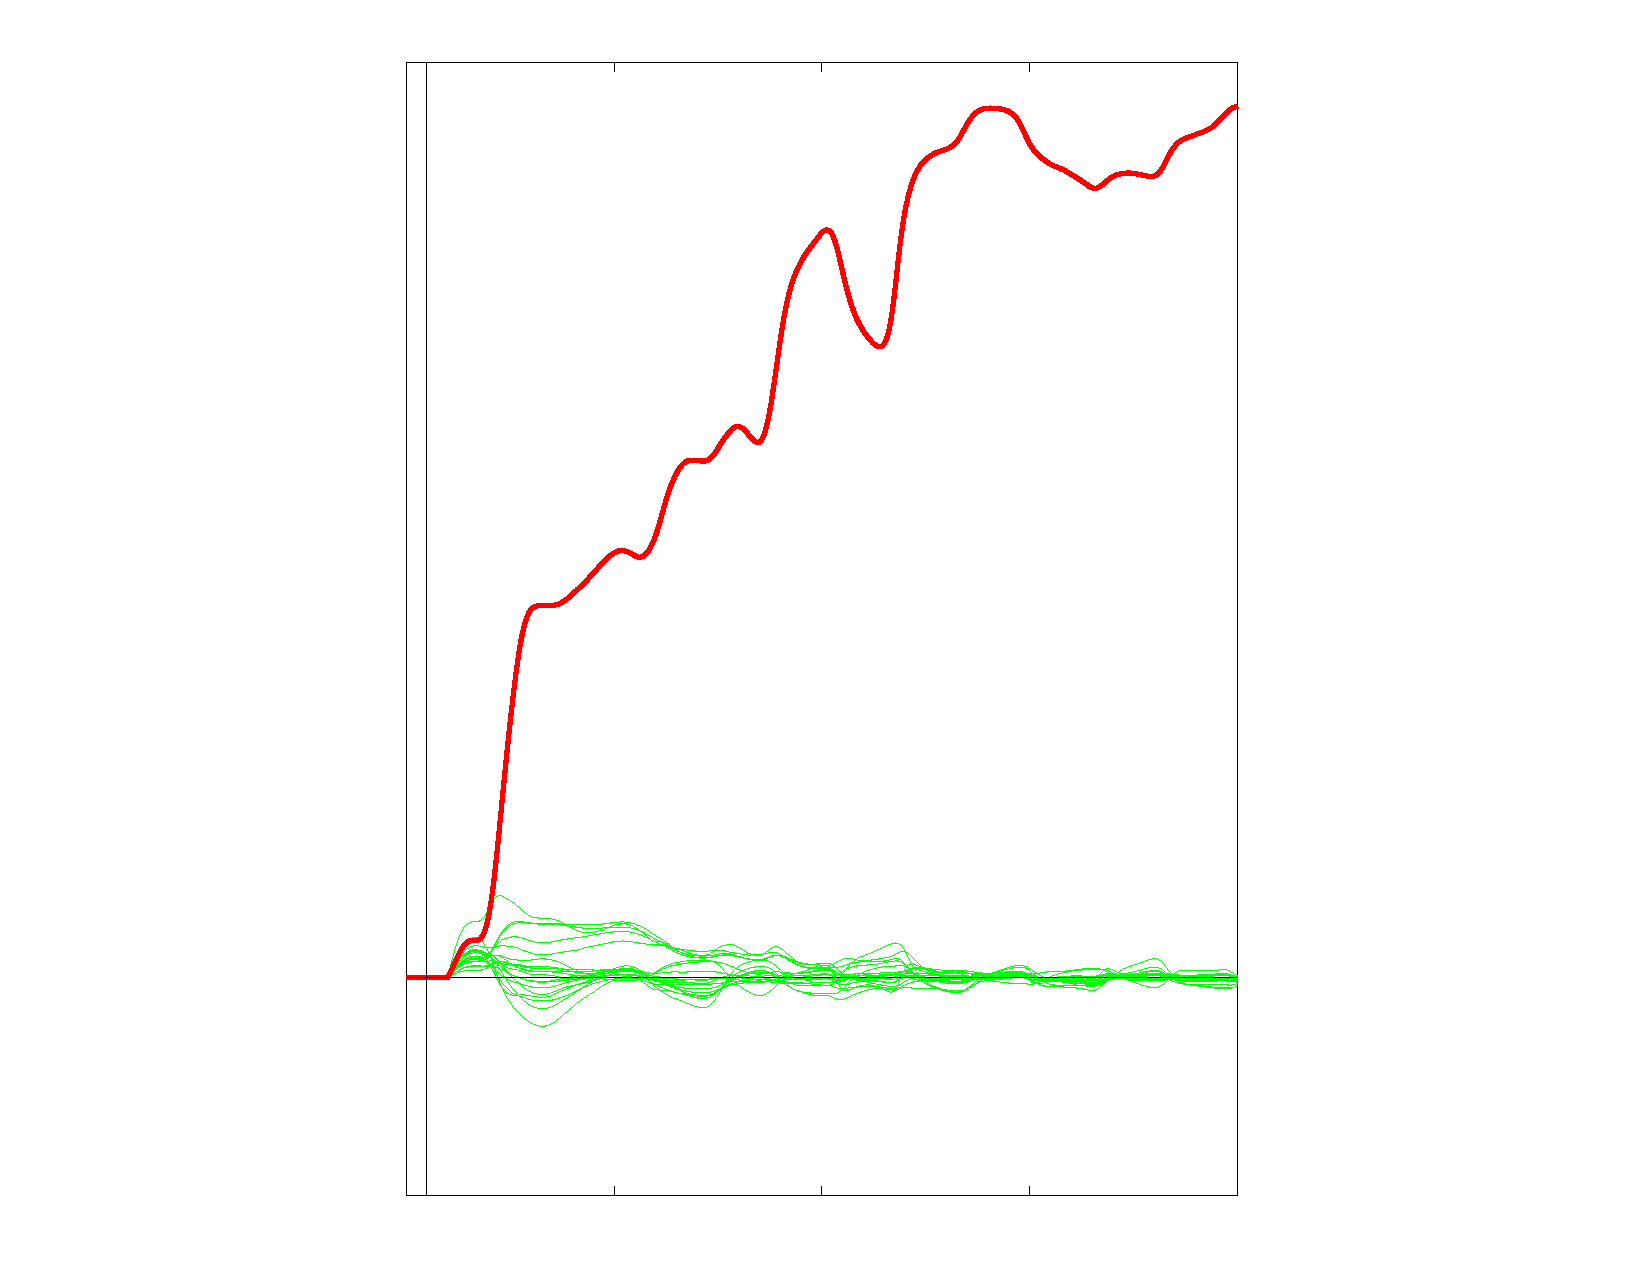
\includegraphics[trim={6.5cm 1cm 5cm 1cm},clip,width=6cm,height=3.5cm]{img/409-clusterSmallWorld-20-addUniform-40-spike-gaussian-Unobserved-rank1-ukf-Xhat}};
\node at (-5.5,-0.25) {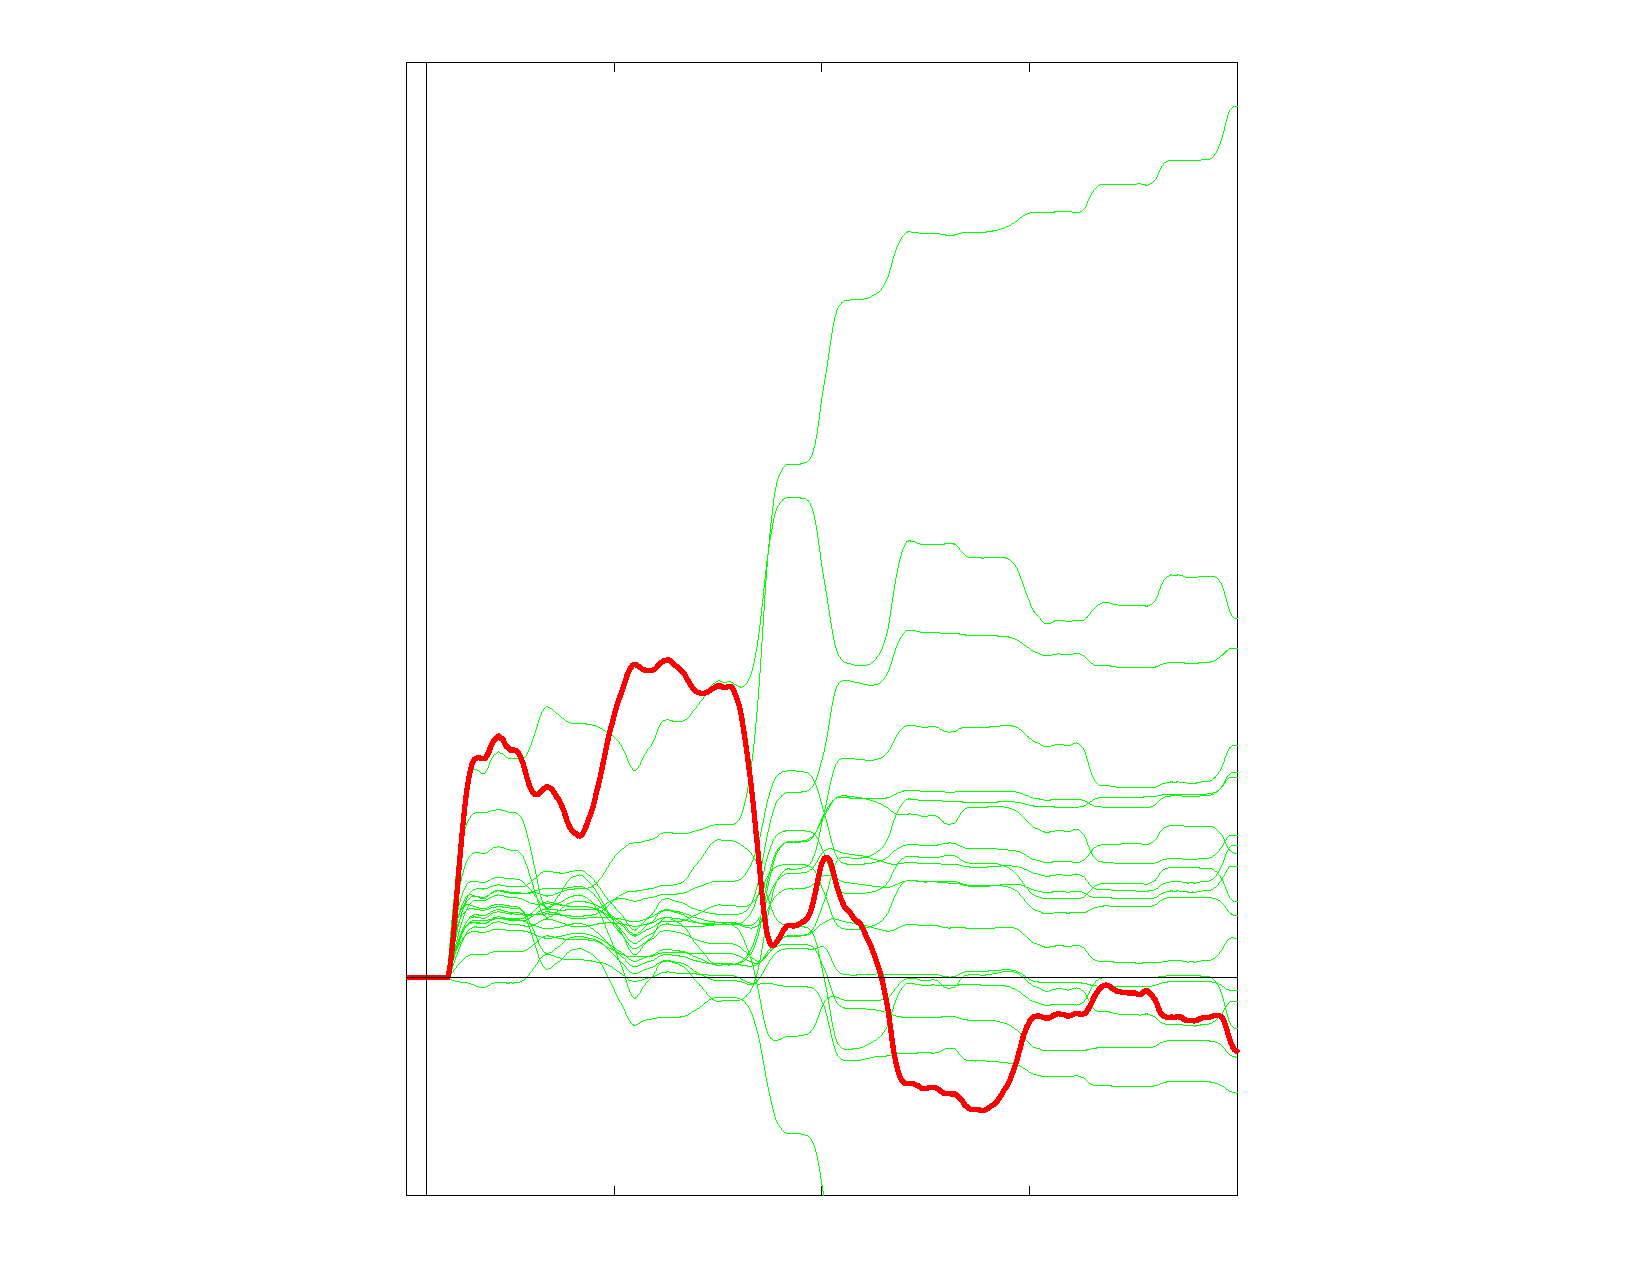
\includegraphics[trim={6.5cm 1cm 5cm 1cm},clip,width=6cm,height=3.5cm]{img/409-clusterSmallWorld-20-addUniform-40-spike-gaussian-Unobserved-fullKL-ukf-Xhat}};
}

\uncover<2>{
\node at (0,-0.25) {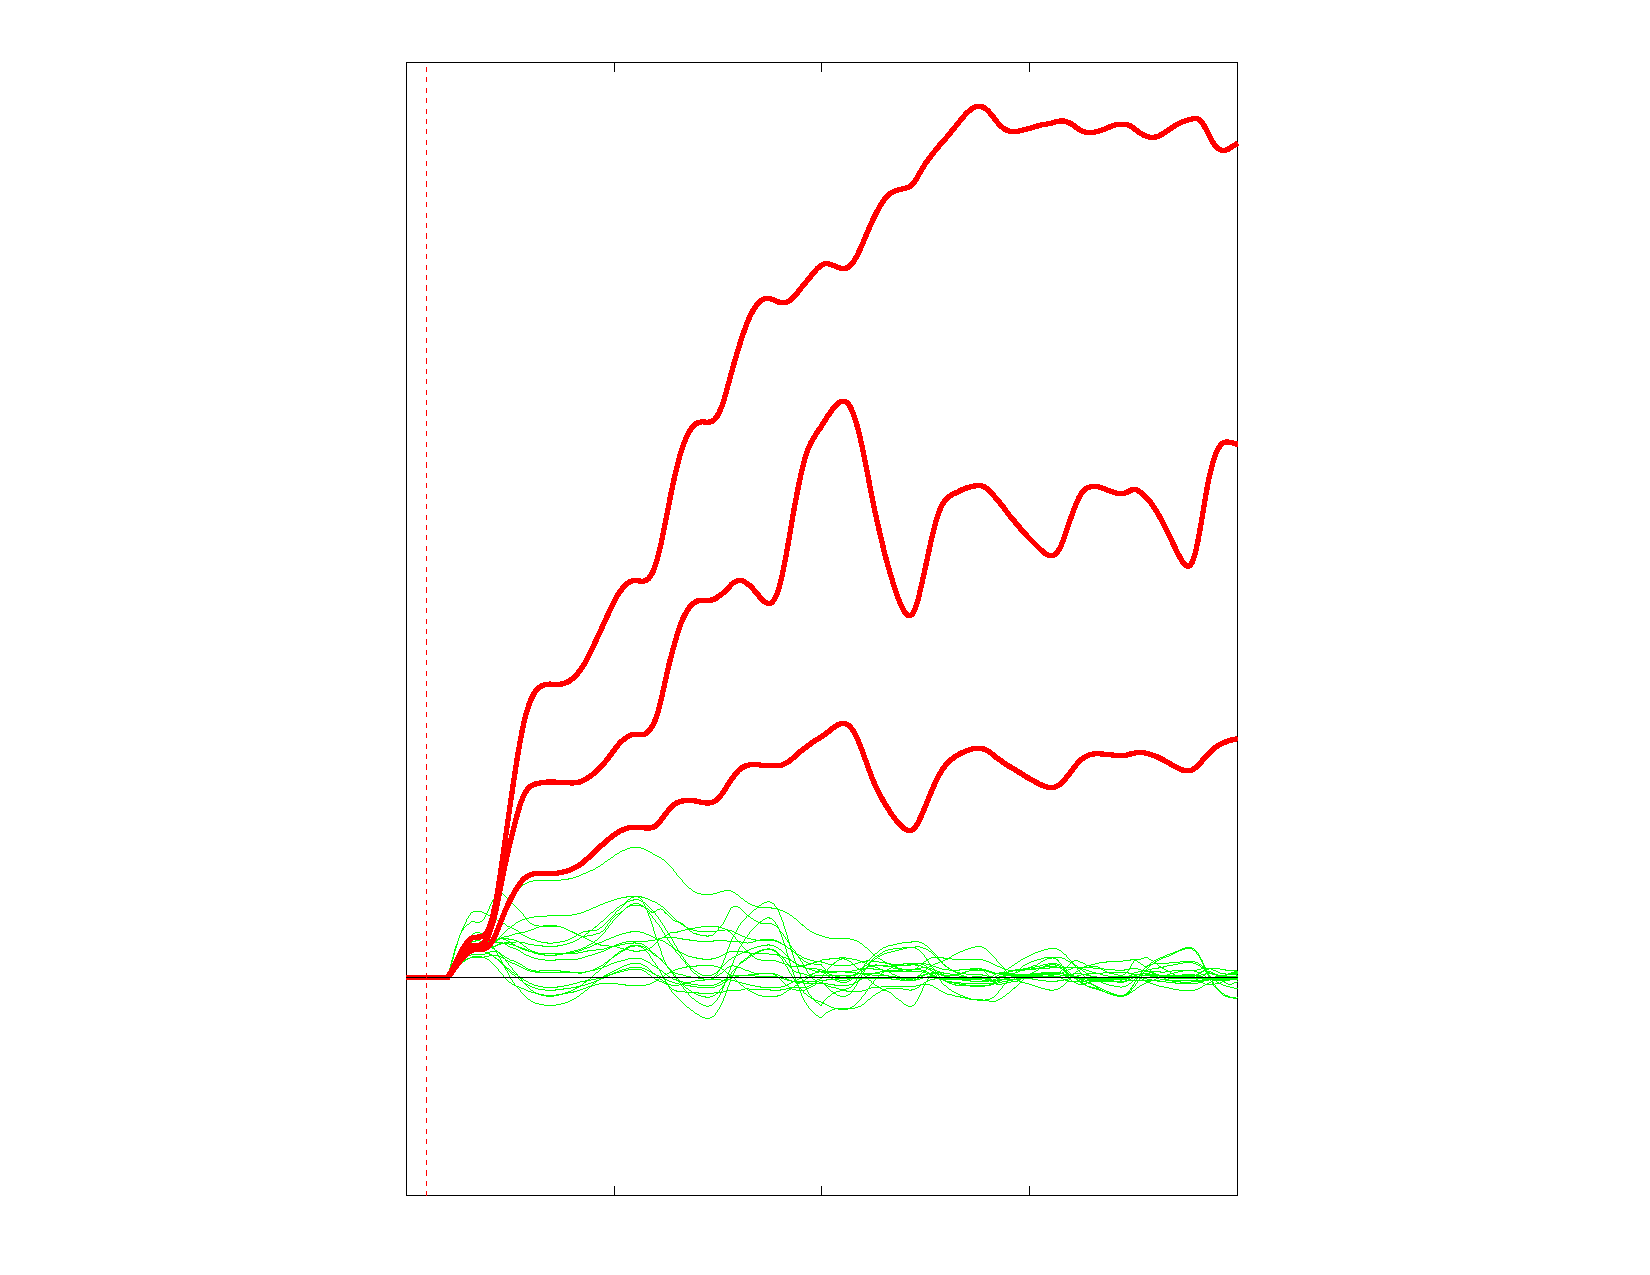
\includegraphics[trim={6.5cm 1cm 5cm 1cm},clip,width=6cm,height=3.5cm]{img/409-clusterSmallWorld-20-addUniform-40-spike3-gaussian-Unobserved-rank1-ukf-Xhat}};
\node at (-5.5,-0.25) {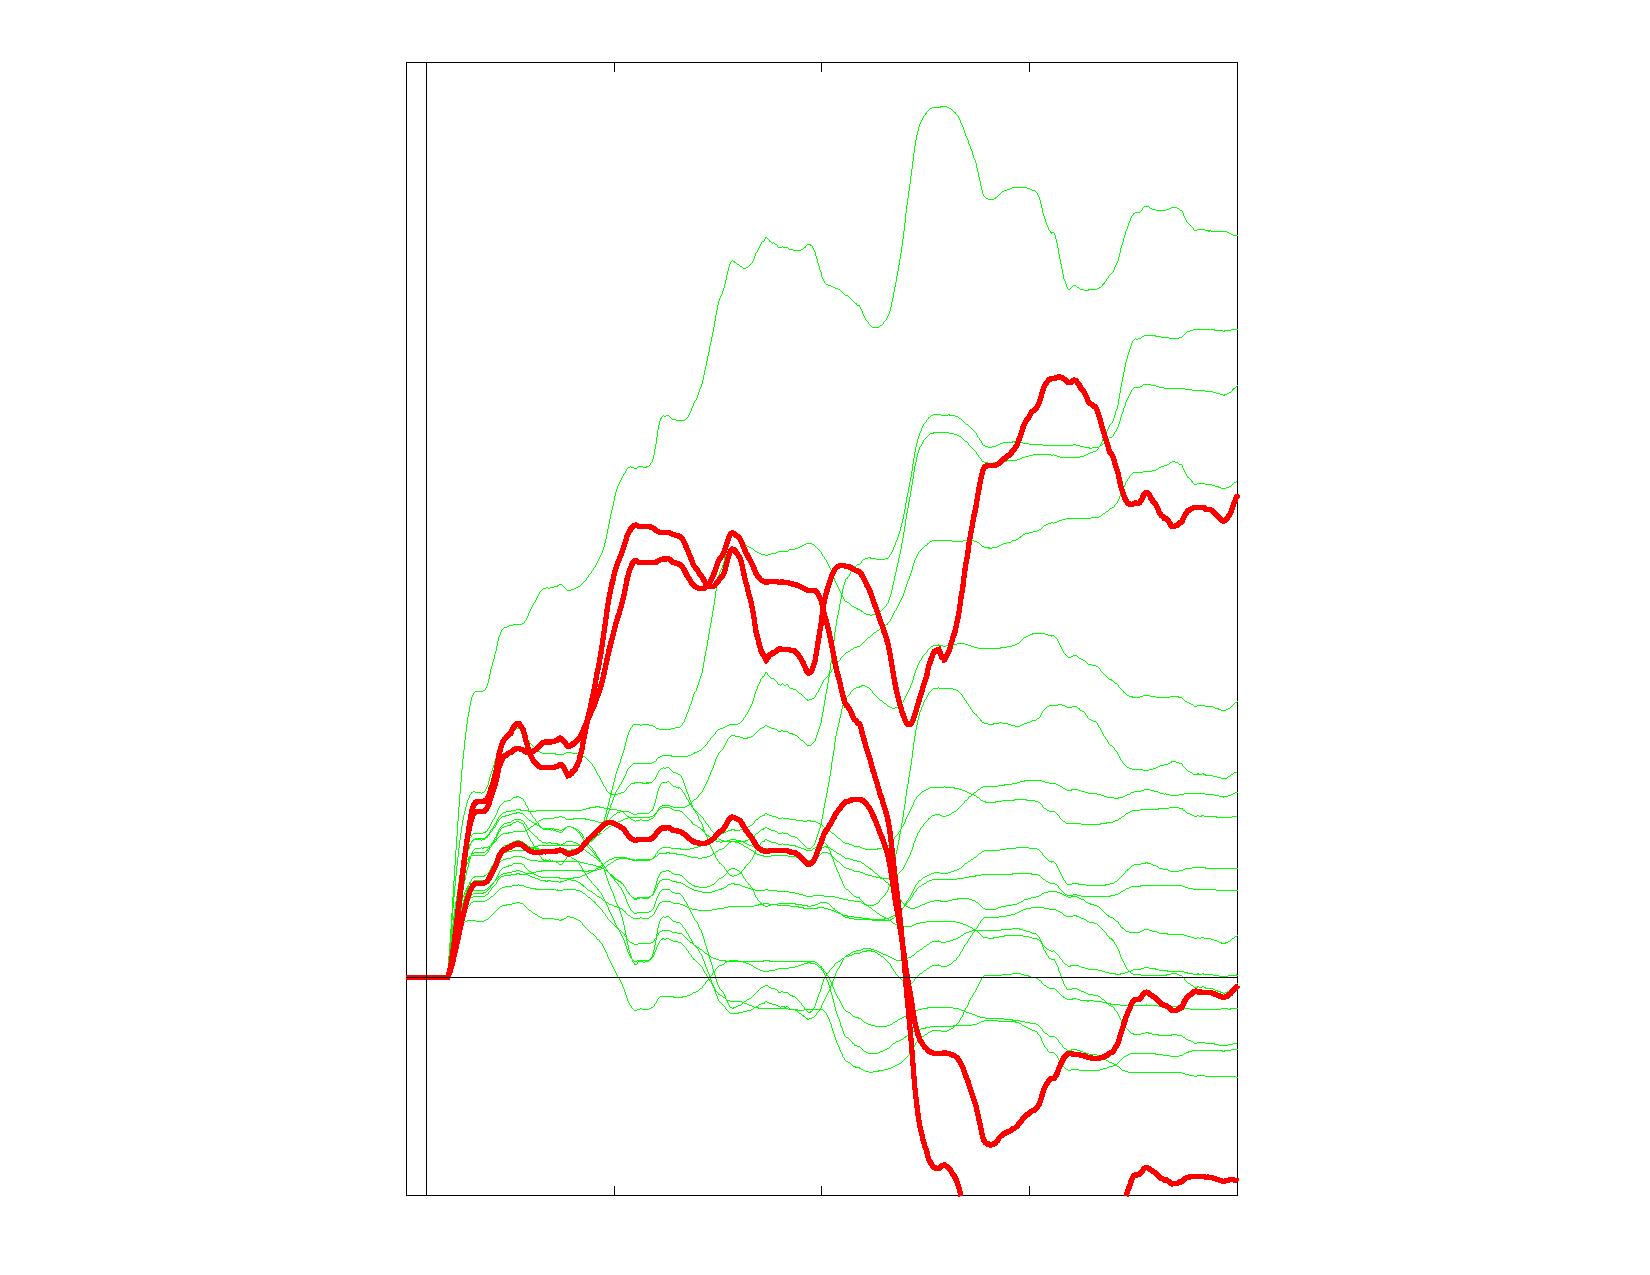
\includegraphics[trim={6.5cm 1cm 5cm 1cm},clip,width=6cm,height=3.5cm]{img/409-clusterSmallWorld-20-addUniform-40-spike3-gaussian-Unobserved-fullKL-ukf-Xhat}};
}

\uncover<3>{
\node at (0,-0.25) {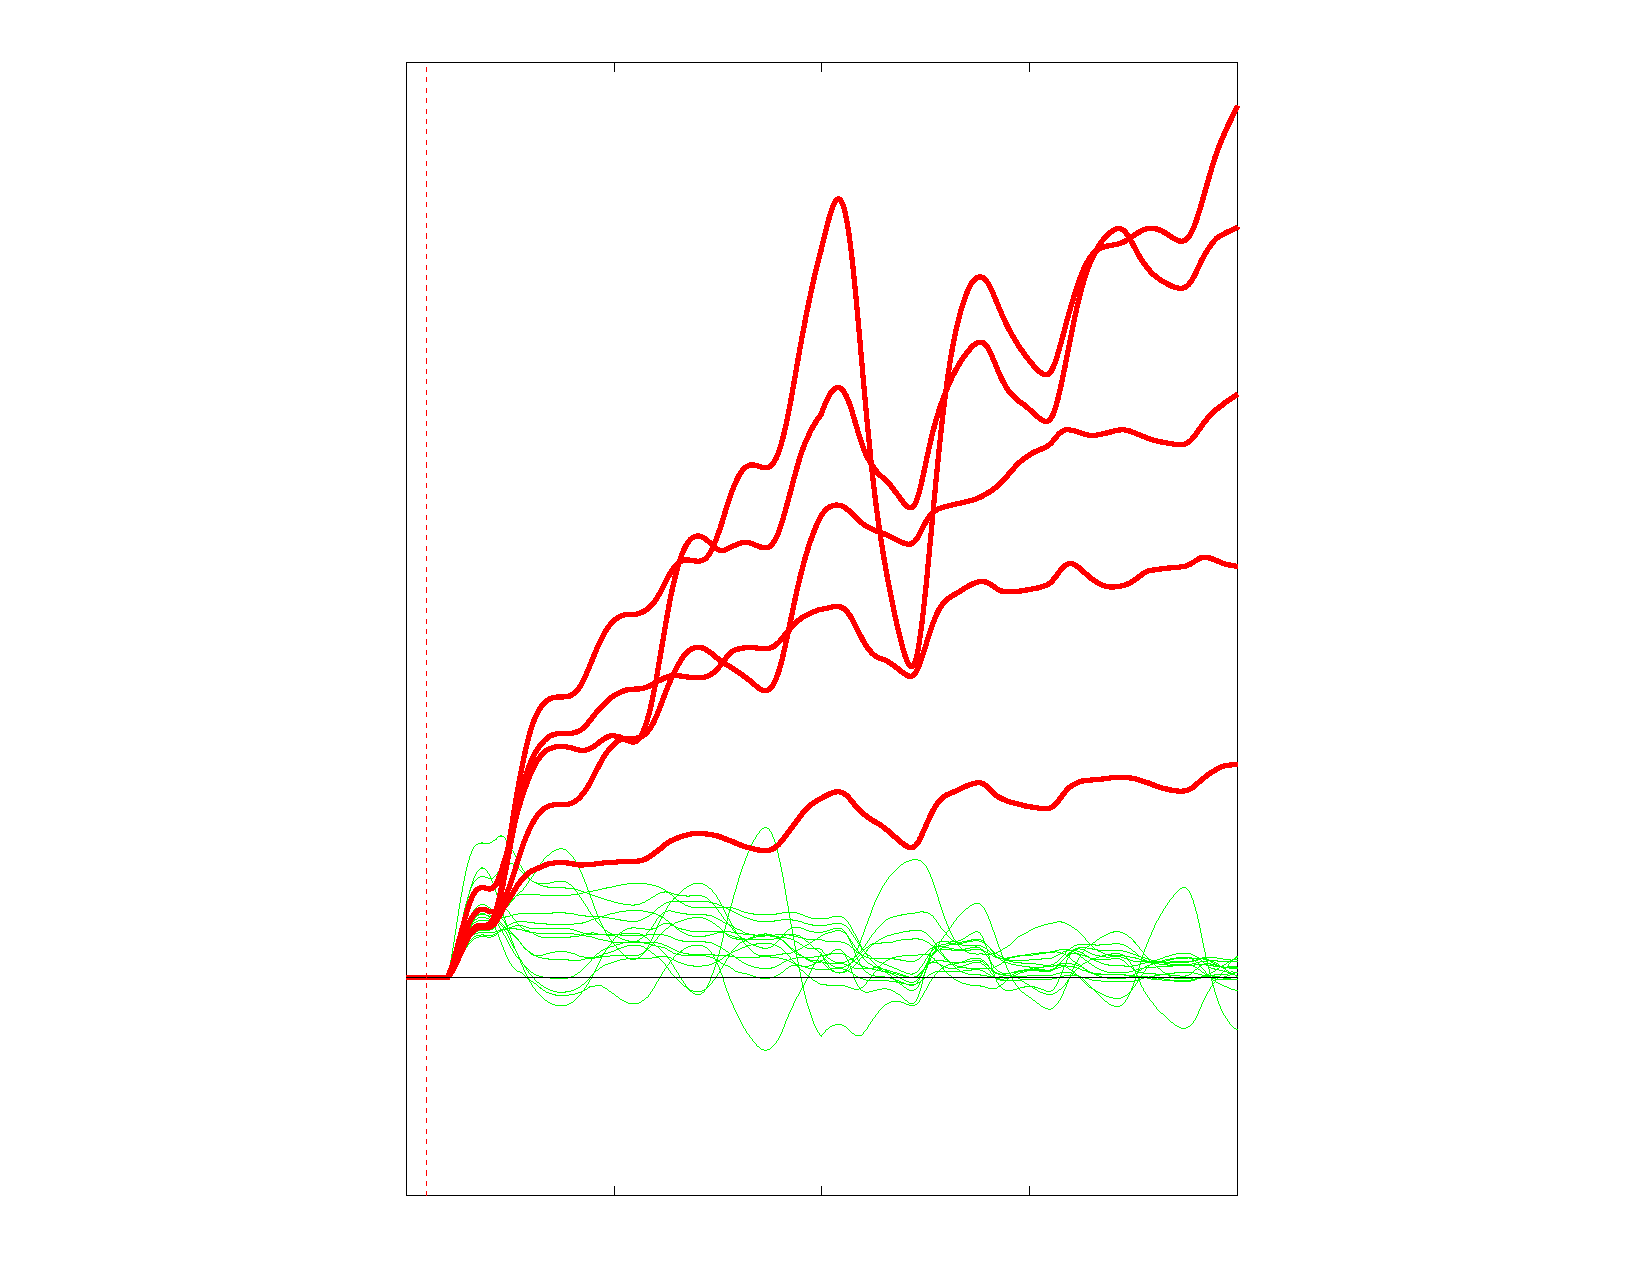
\includegraphics[trim={6.5cm 1cm 5cm 1cm},clip,width=6cm,height=3.5cm]{img/409-clusterSmallWorld-20-addUniform-40-spike5-gaussian-Unobserved-rank1-ukf-Xhat}};
\node at (-5.5,-0.25) {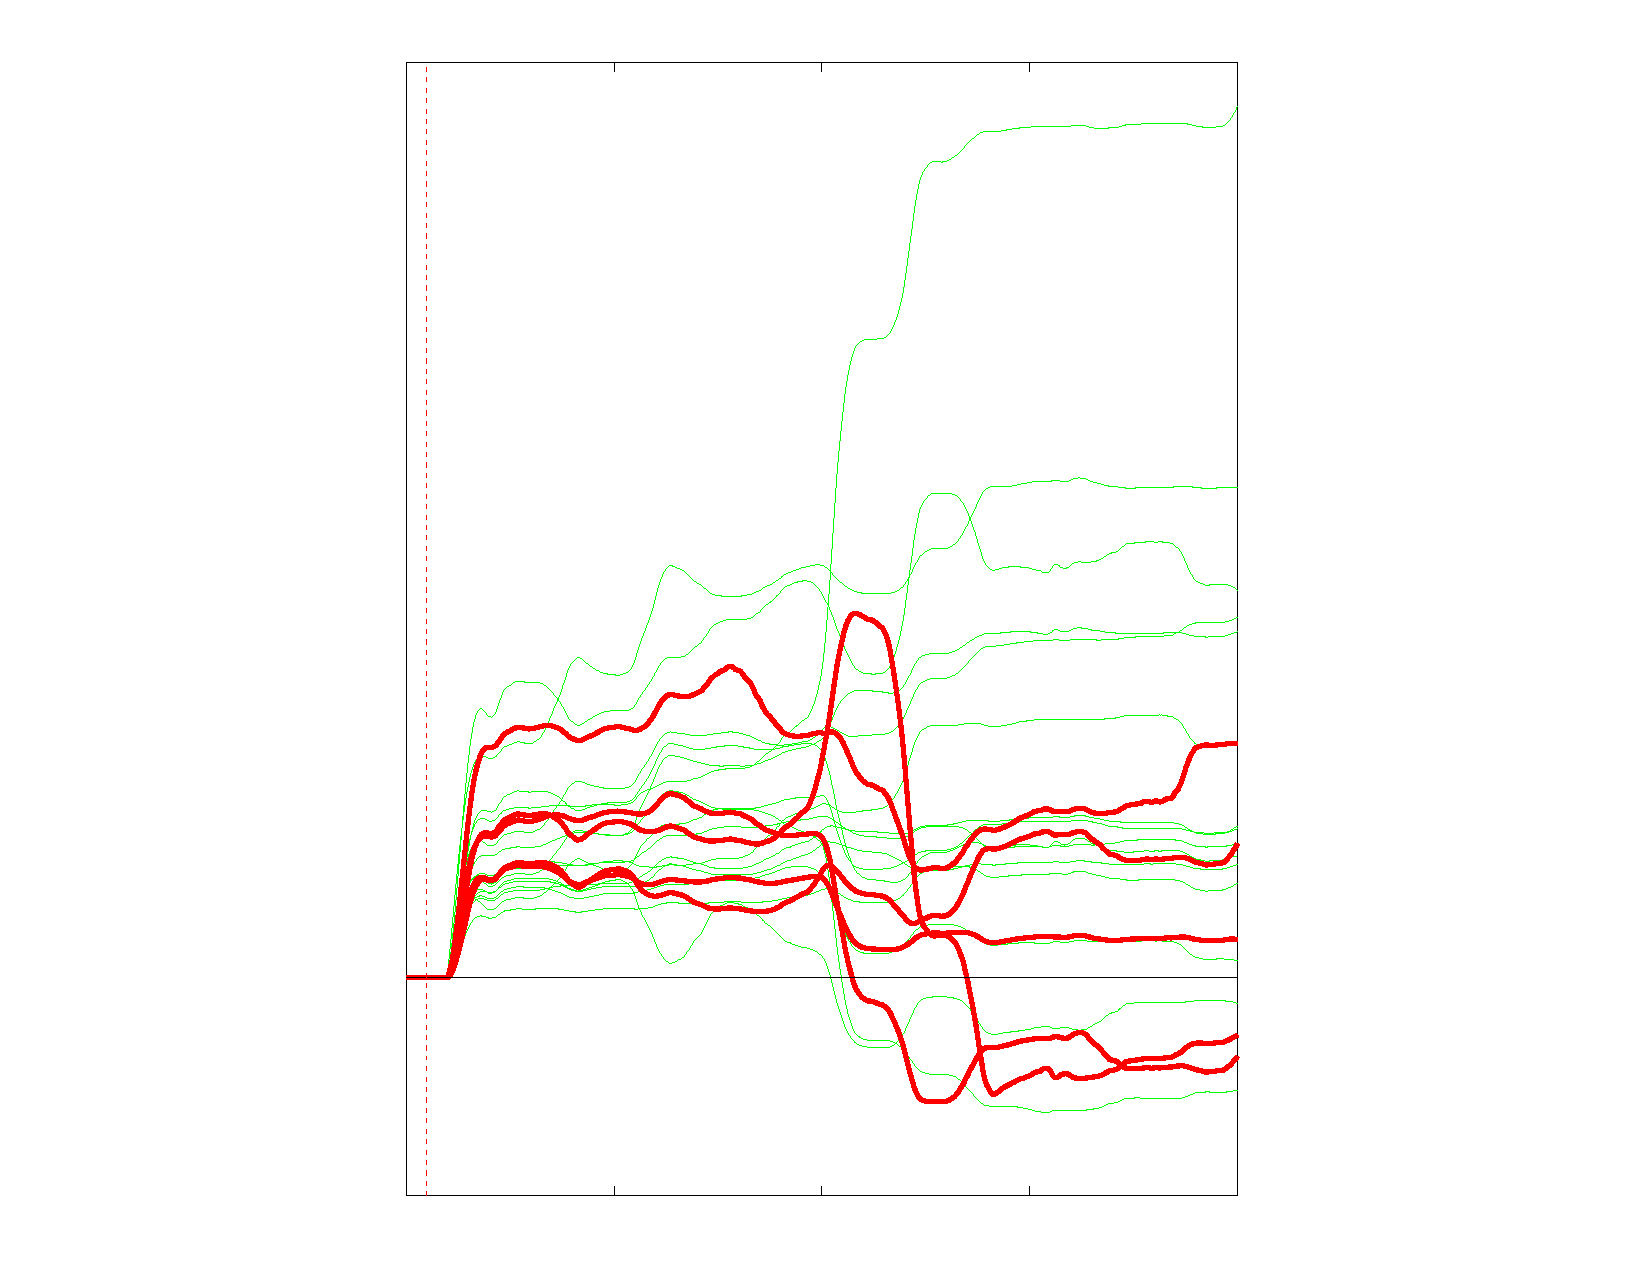
\includegraphics[trim={6.5cm 1cm 5cm 1cm},clip,width=6cm,height=3.5cm]{img/409-clusterSmallWorld-20-addUniform-40-spike5-gaussian-Unobserved-fullKL-ukf-Xhat}};
}

\node at (-5.755,2.0) {full rank $K^{LG}$};
\node at (-0.25,2.0) {rank-1 $K^{LG}$};
%\node at (-0.25,5.75) {3 compromised buses};
%\node at (5.25,5.75) {5 compromised buses};

%\draw (-8.25,-2.65) -- (-7.30,-2.65);
%\draw[->] (-4.2,-2.65) -- (7.75,-2.65);
\node at (-5.75,-2.65) {simulation time (sec)};

\node at (-8.35,-2.25) {0.0};
\node at (-7.05,-2.25) {0.5};
\node at (-5.75,-2.25) {1.0};
\node at (-4.45,-2.25) {1.5};
\node at (-3.25,-2.25) {2.0};

\node at (-6.75,1.25) {attack initiated};
\draw[->,darkgray] (-7.95,1.25) -- (-8.15,1.25);

\node at (-1.5,1.15) {\color{red} compromised };
\node at (-1.5,0.80) {\color{red} buses};
%\draw[->,red] (-6,3.95) -- (-6.15,4.15);

\node at (0.3, -1.6) {\color{darkgreen} uncompromised buses};
%\draw[->,green] (5.25,0.9) -- (5.5,0.8);
\end{tikzpicture}

\vspace{0.0755in}
The \textcolor{red}{red line} should be high and the \textcolor{darkgreen}{green lines} should be low.

\vspace{0.075in}
The rank-1 approximation outperforms the full rank estimator

\vspace{0.075in}
\uncover<2-3> {
    (even when the rank of $K^{LG}>1$)
}
\end{frame}

%%%%%%%%%%%%%%%%%%%%%%%%%%%%%%%%%%%%%%%%%%%%%%%%%%%%%%%%%%%%%%%%%%%%%%%%%%%%%%%%

\begin{frame}{Simulation results (identification accuracy)}

At any timestep $t$, our method has accuracy 1 if all the compromised buses have highest estimated $K^{LG}_t$ entries; otherwise the method has accuracy 0

\vspace{0.075in}
Repeat our experiment over 100 random configurations

\begin{center}
\scalebox{0.8}{
\begin{tikzpicture}
%\small
\node at (-0.1,0) {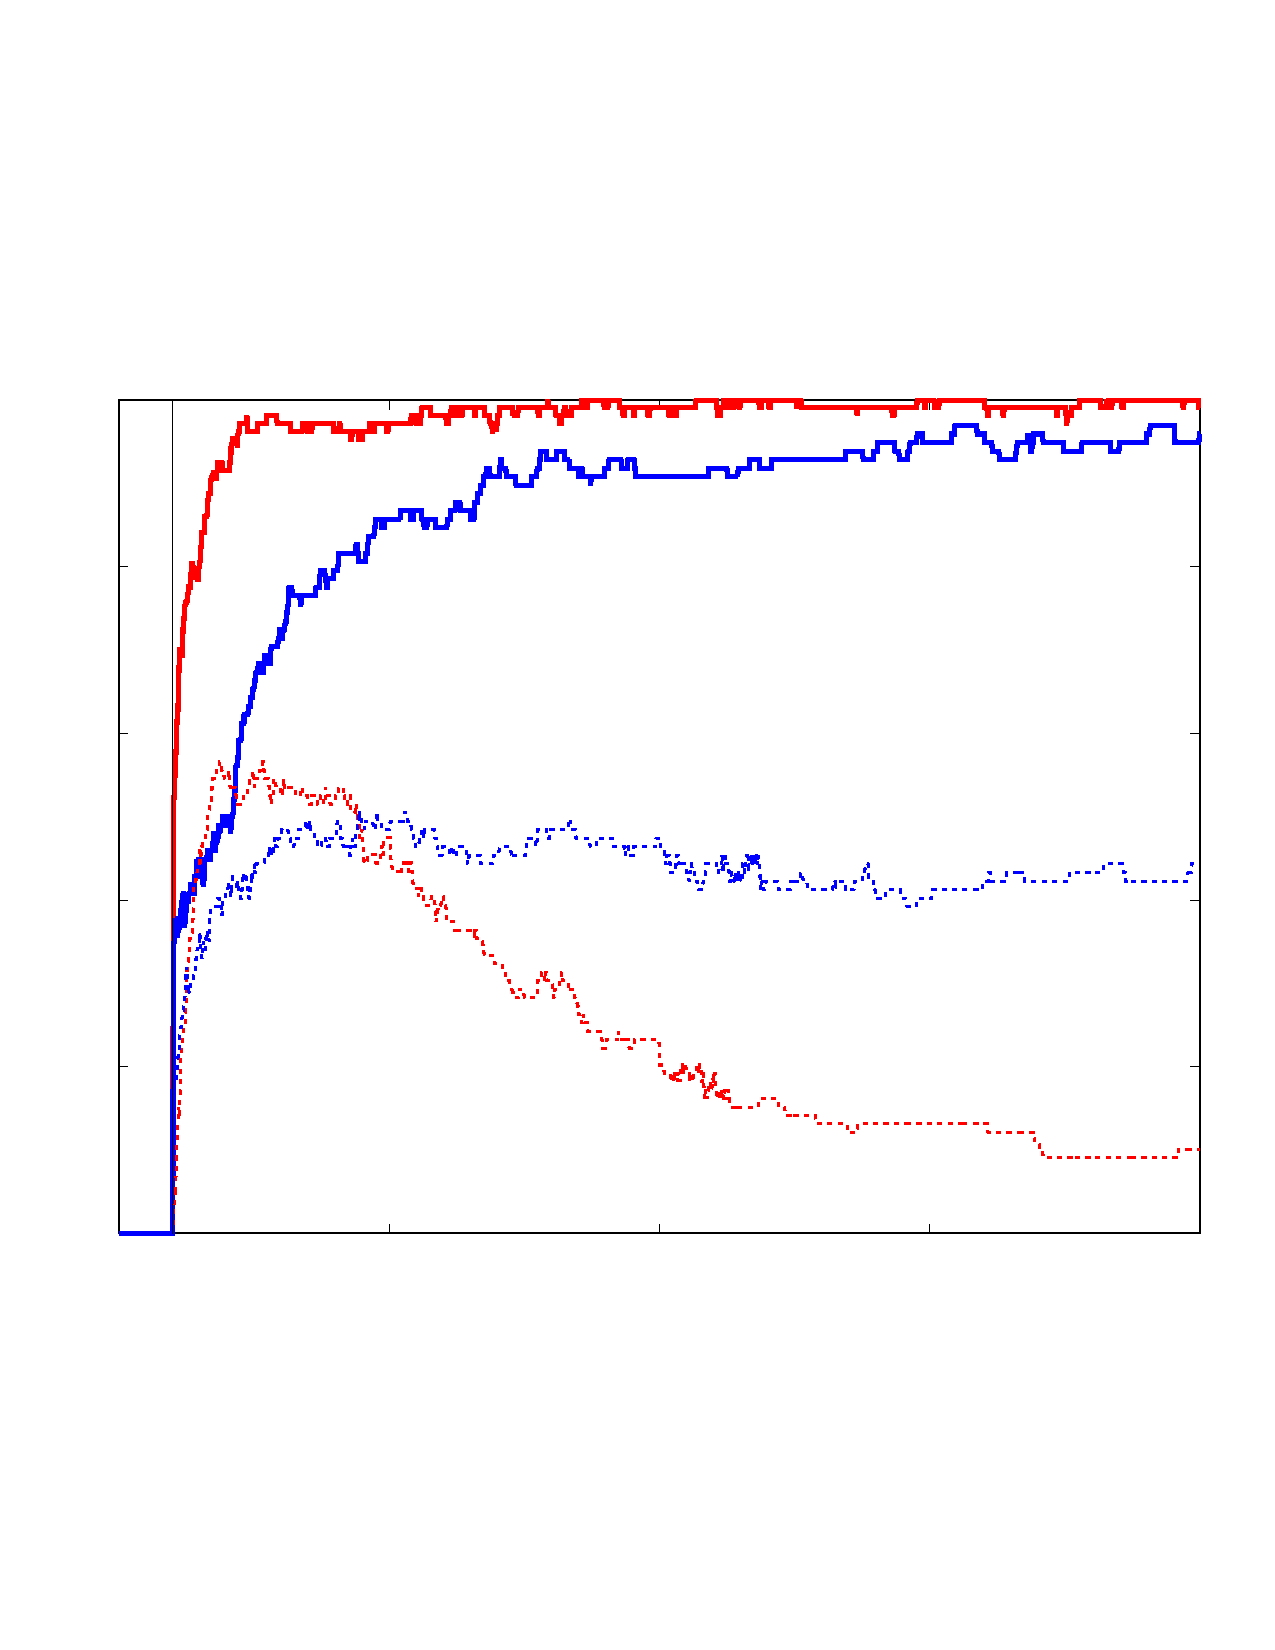
\includegraphics[trim={2cm 5cm 1cm 5cm},clip,width=7.2cm,height=7cm]{img/accuracy}};
\node at (0.0,-3.5) {simulation time (sec)};
\node at (-4.7,0) {\rotatebox{90}{accuracy of $\alpha_t$}};

\node at (-3.65,-3) {0.0};
\node at (-1.85,-3) {0.5};
\node at (-0.1,-3) {1.0};
\node at (1.65,-3) {1.5};
\node at (3.45,-3) {2.0};

\node at (-4.1,-2.7) { 0.0 };
\node at (-4.1,-1.6) { 0.2 };
\node at (-4.1,-0.5) { 0.4 };
\node at (-4.1,0.55) { 0.6 };
\node at (-4.1,1.65) { 0.8 };
\node at (-4.1,2.8) { 1.0 };

\node at (-1.7,-2.2) {\color{darkgray}attack initiated};
\draw[darkgray,->] (-2.9,-2.2) -- (-3.3,-2.2);

\node at (2,-1.5) {\color{red}\begin{tabular}{c}full $K^{LG}$\\1 compromised bus\end{tabular}};

\node at (2,0.25) {\color{blue}\begin{tabular}{c}full $K^{LG}$\\5 compromised buses\end{tabular}};

\node at (2,1.95) {\color{blue}\begin{tabular}{c}rank-1 $K^{LG}$\\5 compromised buses\end{tabular}};

\node at (-1.75,3.25) {\color{red}\begin{tabular}{c}rank-1 $K^{LG}$\\1 compromised bus\end{tabular}};

\end{tikzpicture}
}
\end{center}
\end{frame}
